\documentclass[a4paper, 12pt]{article} % Font size (can be 10pt, 11pt or 12pt) and paper size (remove a4paper for US letter paper)
\usepackage[margin=3cm]{geometry}

\usepackage[protrusion=true,expansion=true]{microtype} % Better typography
\usepackage{graphicx} % Required for including pictures
\usepackage{wrapfig} % Allows in-line images
\usepackage{natbib}
\usepackage{float}
\usepackage{parskip}
\usepackage{amssymb}
\usepackage{amsmath}
\setcitestyle{authoryear, open={(},close={)},citesep={,},aysep=}
\usepackage{hyperref}
\usepackage[utf8]{inputenc}
\usepackage[ddmmyyyy]{datetime}

\usepackage{mathpazo} % Use the Palatino font
\usepackage[T1]{fontenc} % Required for accented characters

\linespread{1.3} % Change line spacing here, Palatino benefits from a slight increase by default

\def\UrlBreaks{\do\/\do-}
\makeatletter
\renewcommand\@biblabel[1]{\textbf{#1.}} % Change the square brackets for each bibliography item from '[1]' to '1.'
\renewcommand{\@listI}{\itemsep=0pt} % Reduce the space between items in the itemize and enumerate environments and the bibliography
\renewcommand{\dateseparator}{.}

\renewcommand{\maketitle}{ % Customize the title - do not edit title and author name here, see the TITLE block below
    \begin{center} % Right align
        {\LARGE\@title} % Increase the font size of the title

        \vspace{30pt} % Some vertical space between the title and author name

        {\@author} % Author name

        \vspace{30pt} % Some vertical space between the author block and abstract
    \end{center}
}

%----------------------------------------------------------------------------------------
%   TITLE
%----------------------------------------------------------------------------------------

\title{Restoring axial resolution using a 2D/3D deep convolution neuronal network}

\author{
    \large{Joey Zenhäusern}\\ % Author
    \small{
        \texttt{Section of Computer Science}
    }
} % Institution


%----------------------------------------------------------------------------------------

\begin{document}
\maketitle % Print the title section

\begin{center}
    \fbox{%
        \parbox{\textwidth}{%
            \vspace{10pt}
            \begin{center}
                Semester Project Master\\
                12 Credits\\
                Biomedical Imaging Laboratory\\
                \vspace{10pt}
                Supervision:\\
                Prof. Michael Unser\\
                Dr. Daniel Sage\\
                Dr. Kyong Jin\\
                \vspace{10pt}
                Submission date: \today
            \end{center}
            \vspace{10pt}
        }%
    }
\end{center}

\vspace{20pt}

\begin{center}
    Lausanne, Spring Semester 2018
\end{center}
\begin{figure}[H]
    \centering
    
\includegraphics[width=0.7\textwidth]{./figures/epfl.png}
\end{figure}

\newpage

\tableofcontents
\newpage

\section{Introduction}
In 3D fluorescence microscopy, the axial resolution (Z-axis) is often lower than the lateral resolution (optical plane XY), due to the elongation of the point spread function along the Z-axis as well as mechanical limitations in fluorescence microscopy. This non-isotropic resolution penalizes the global resolution of the biological structures. The conventional way to expand the size is to interpolate in the Z axis, which creates blurry 3D images without recovering any structure. In this project, we attempt to recover the axial resolution by employing a deep learning method. Because there is no ground truth available, we implement a 2D approach in which the XY images are split up into patches and then fed to a deep convolutional neuronal network (CNN) with a U-Net \citep{unet} structure. The goal is for the network to learn a mapping between the low and the high resolution patches (XY plane), in order to apply it to XZ and XY images and hence recover full isotropic resolution.

The U-Net architecture, initially proposed for image segmentation, is depicted in Figure~\ref{fig:unet}. It has been used by \citet{WEIGERT2017} for the same purpose as we intend to use it in this project, yielding very promising results. The architecture consists of a contracting path followed by a more or less symmetric expanding path, in which the learned features are upsampled and combined with higher resolution information from the contracting path.

\begin{figure}[h]
    \begin{center}
        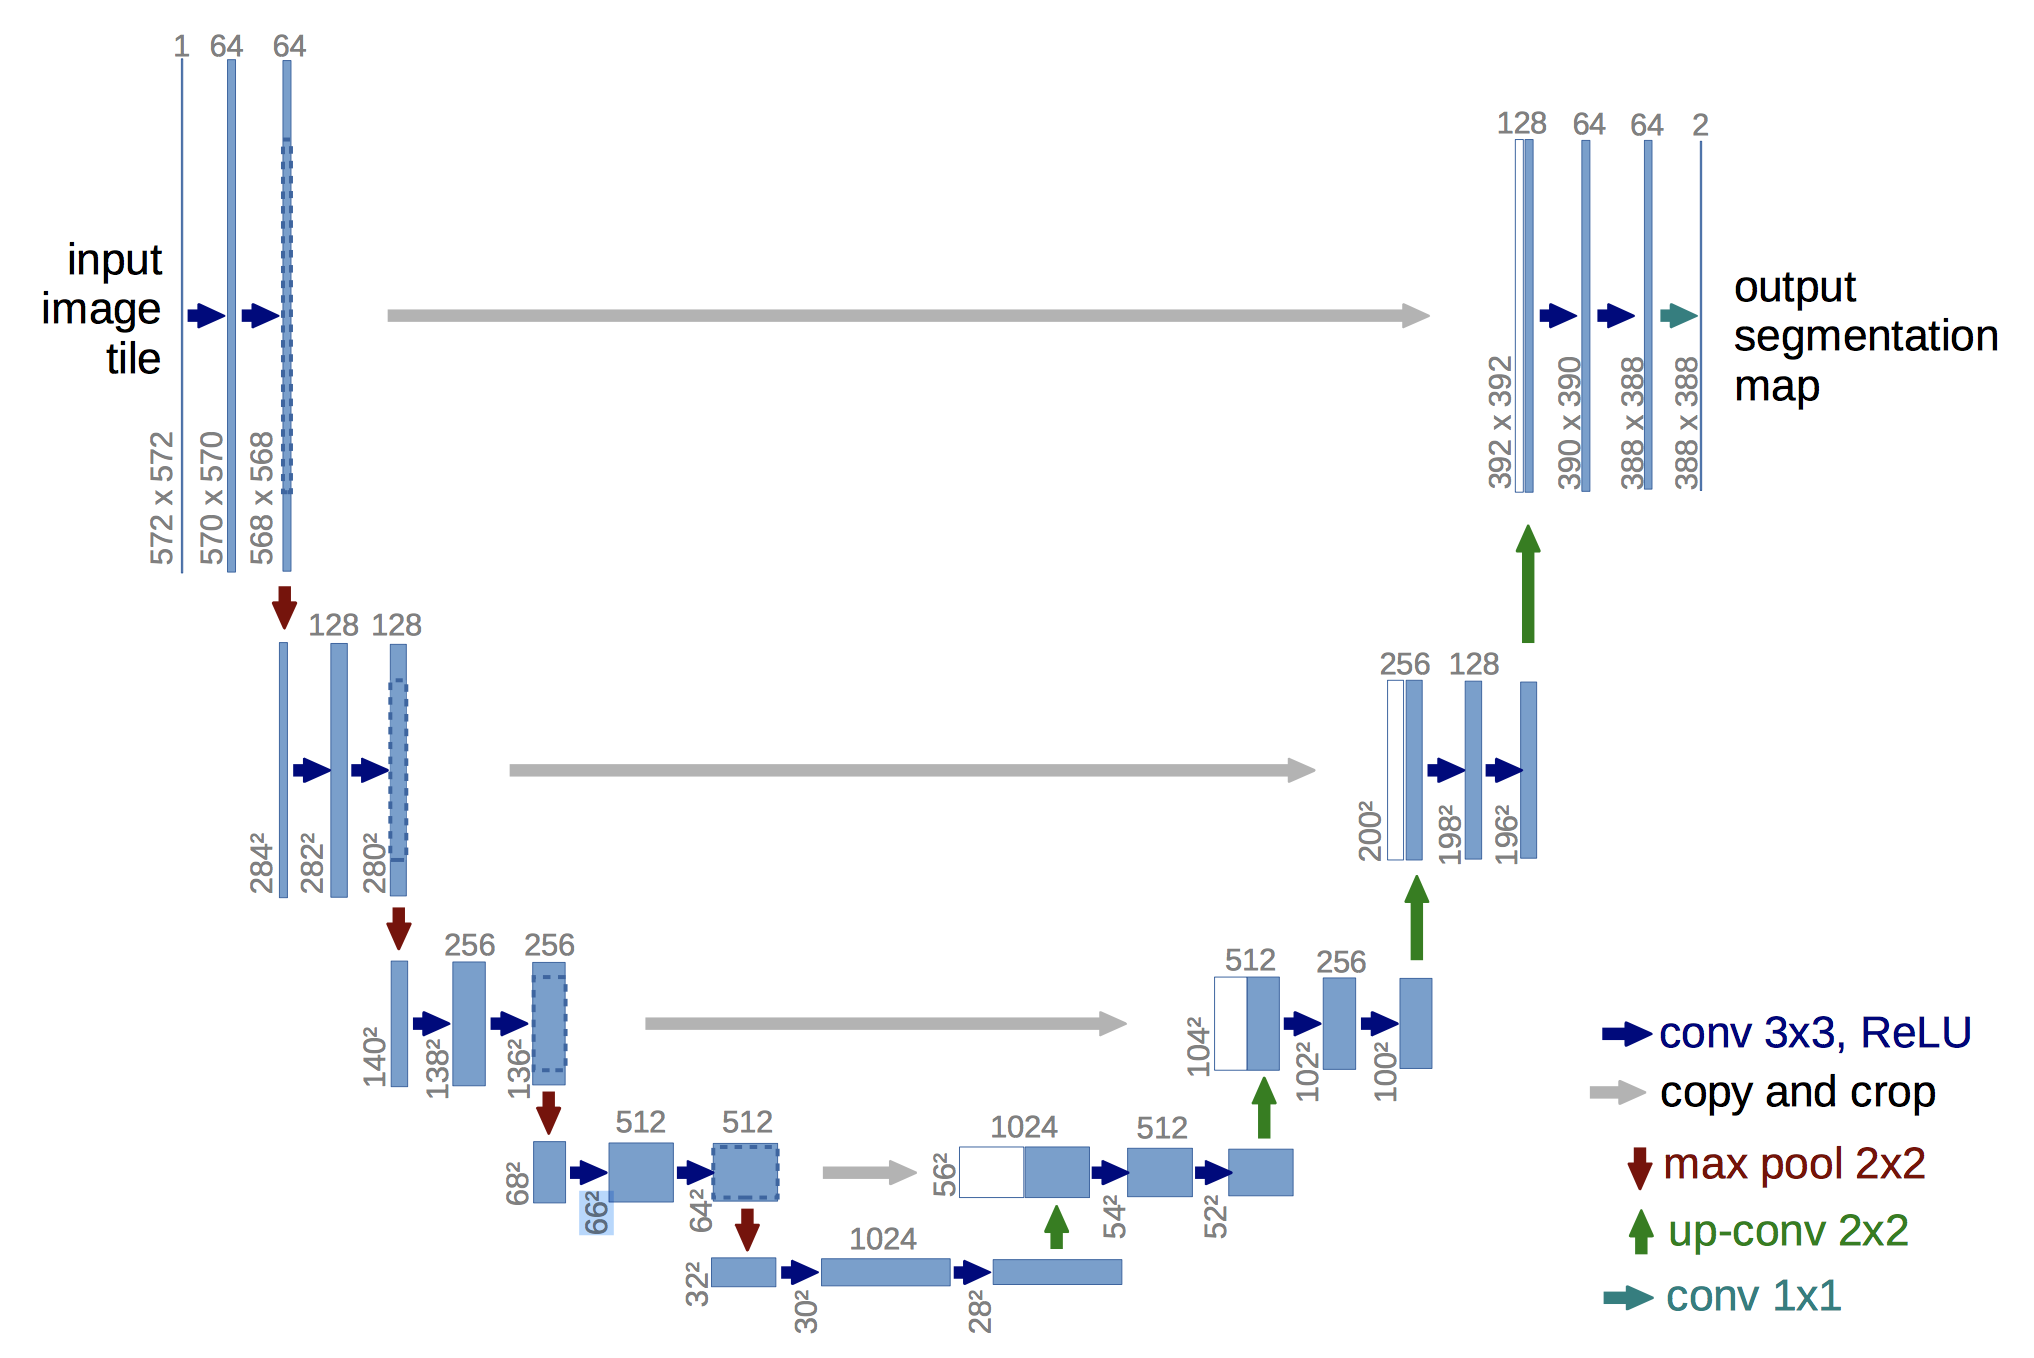
\includegraphics[width=0.8\columnwidth]{figures/unet.png}
        \caption{U-Net architecture from~\cite{unet}\label{fig:unet}. Blue boxes correspond to multi-channel feature maps with the number of channels written on top. White boxes are copied feature maps and arrows represent the different operations.}
    \end{center}
\end{figure}

\section{Methodology}
\subsection{Implementation}
All code is written in Python 3, using the Tensorflow \citep{tensorflow2015-whitepaper} framework, as well as the Python libraries NumPy and Pillow. The training procedure is launched by executing \texttt{src/tf\_restore\_axial\_res.py}. A number of flags may be passed in order to set parameters such as:

\begin{itemize}
    \item \texttt{batch\_size}: Batch size for training and prediction
    \item \texttt{patch\_size}: Size of training patches
    \item \texttt{stride}: Distance between extracted training patches
    \item \texttt{num\_epoch}: Number of epochs to perform during training
    \item \texttt{num\_layers}: Number of layers in the U-net architecture.
    \item \texttt{conv\_size}: Size of convolution filters
    \item \texttt{dilation\_size}: Size of dilated convolution filters
    \item \texttt{full\_prediction}: Whether or not to generate full prediction after network is fully trained
    \item \texttt{learning\_rate}: Learning rate for the Adam optimizer
    \item \texttt{dropout}: Dropout rate of the network
    \item \texttt{data}: Path to training data
    \item \texttt{k\_factor}: Factor by which axial resolution will be increased
    \item \texttt{gpu}: Identifying number of GPU to use for training
\end{itemize}

In a first step, the provided image is loaded and the lateral image layers are split up into patches, providing the ground truth for the training step. In order to obtain the training patches, a copy of the tensor containing the ground truth patches will then be downscaled by only keeping every $k$-th row in every patch, where $k$ is the \texttt{k\_factor} mentioned above. Note that the number of training patches that can be obtained this way is $k$ times the number of ground truth patches obtained in the initial extraction, since there are $k$ starting positions to keep every $k$-th row in a patch. This also implies that training time per epoch (one iteration of every patch in the dataset) for higher $k$ will increase in proportion to $k$. The training patches are subsequently resized to their original square size by means of a bicubic interpolation.

The optimization step is performed by the Adam optimizer \citep{kingma2014adam}. We have set the loss function to be the pixel wise negative peak signal-to-noise ratio between the ground truth patches ($o(x, y)$) and the predicted patches ($p(x, y)$) as stated in Equation~\ref{eq:loss}.

% describe loss function
\begin{equation}\label{eq:loss}
    \mathcal{L} = -20 \cdot \big[ \log_{10}[\max o(x, y)] - \log_{10}[\sqrt{\text{MSE(o(x, y), p(x, y))}}] \big]
\end{equation}

where $\max()$ is the maximum possible pixel value of the given image and $\text{MSE()}$ is the mean squared error between two images.

\subsection{Network Architecture}
\subsubsection{Baseline Network}\label{sec:baseline}
We started out with the \textit{Isonet-2} architecture, described in \citet{WEIGERT2017} as follows:
\begin{equation}\label{eq:base-model}
    C_{16, 7, 7} - M_{2, 2} - C_{32, 7, 7} - M_{2, 2} - C_{64, 7, 7} - U_{2, 2} - C_{32, 7, 7} - U_{2, 2} - C_{16, 7, 7} - C_{1, 1, 1}
\end{equation}
where:
\begin{align}\label{network-params}
    C_{n, w, h}:\quad &\text{Convolutional layer with $n$ filters of size $(w, h)$}\\
    M_{p, q}:\quad &\text{Max pooling layer with a subsample factor of $(p, q)$}\\
    U_{p, q}:\quad &\text{Upsampling layer with a subsample factor of $(p, q)$}
\end{align}

In addition to the above, each convolution layer is followed by a ReLu activation layer, as well as a dropout layer. To avoid some patch size restrictions we use zero padding for convolutions in the neural network. This allows us to get output patches that have the same dimensions as the input patches from the network.

\subsubsection{Dilated Convolution}
For conventional convolution layers with a filter size of $(w \times h)$, as used in the network described in the previous section, the receptive field only grows linearly with the increase of the filter sizes $w$ and $h$. This can be problematic, as the memory requirements during training grow in proportion to $k^2$ assuming a $k \times k$ filter size and computational cost increases as well. One possible solution to this is to use dilated convolutional filters \citep{ferenc-dilated}. A dilated convolution on a 2D input can be seen as a convolution with stride $(p, q)$, in the case where $p=2, q=2$ this filter would hence have a receptive field of $7 \times 7$ as can bee seen in Figure~\ref{fig:dilated}.
\begin{figure}[h]
    \center%
    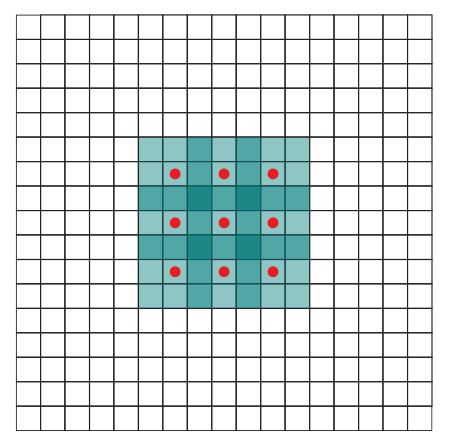
\includegraphics[width=0.3\columnwidth]{figures/dilated.png}
    \caption{Dilated convolution filter from~\cite{ferenc-dilated}}\label{fig:dilated}
\end{figure}

\subsubsection{Increasing Network Depth}
A different approach to reduce memory usage while maintaining a similar receptive field is to increase the depth of the network. If we consider the depth of a convolutional neural network to be the number of convolution layers (excluding the last layer which is the output layer) the Isonet-2 model has a depth of 5. This number can easily be increased by the parameter \texttt{num\_layers}, setting it to $k$ will result in $2k-1$ layers. Each increment of $k$ adds the necessary layers on both the expanding and the contracting part of the U-net architecture. According to \citet{depth} this should allow us to decrease the filter size on each level (and thereby the memory consumption) while maintaining or even improving the model's performance.

\subsection{Hyperparameter Optimization}
Extensive testing (see \ref{sec:results}) has shown that the performance of the network is very sensitive to the hyperparameters in the training procedure. We have set the learning rate and the epsilon parameter for the Adam optimizer to $10^{-3}$, which appears to yield good convergence rates. However, due to the fact that the training process operates on randomized batches of data, the training $PSNR$-loss varies very strongly (see Figure~\ref{fig:noisy-training}) and has to be smoothed significantly in order to recognize the trend. Increasing the batch size as far as the available GPU memory permits alleviates this effect somewhat.

\begin{figure}[h]
    \center%
    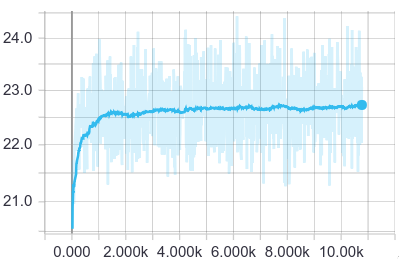
\includegraphics[width=0.4\columnwidth]{./figures/noisy-training.png}
    \caption{Training loss (displayed as the positive PSNR) taken from tensorboard after 30 epochs, x-axis shows steps where a step is the processing of one batch, unsmoothed in bright blue, smoothed (factor 0.99) in dark blue.}\label{fig:noisy-training}
\end{figure}


Many convolutional neural networks use dropout layers to counteract overfitting in exchange for slower convergence and potentially reduced accuracy. In our case, the patches we aim to finally apply the trained model to, are by assumption very similar to the patches that were encountered during training. Also, at this stage in the project we only train on one dataset, to apply the model on the same dataset but on the axial direction. Based on this, we might prioritize the higher accuracy and faster convergence which a lower dropout (or high dropout keep) probability offers, over its potentially regularizing effect, the downside being that the model has to be retrained for every image, or that images have to be very similar to apply a pretrained model.

\section{Results}\label{sec:results}
\subsection{Synthetic Data}
The synthetic dataset which was used to evaluate the performance of the different network architectures and their hyperparameters was generated in a simulator implemented in Java. It generates cells of a c-elegans (a type of roundworm) with different degrees of shape deformation, gaussian noise and poisson noise. For the purpose of this project, we used a dataset with 50\% shape deformation, a gaussian noise intensity of 100 as well as poisson noise with parameter 1. The synthetic data is fully isotropic, which means we have an axial ground truth available to evaluate the perfomance of our models.

\begin{table}[h]
\centering
\begin{tabular}{c | c | c | c | c | c}
 \#  & dilated\_size & conv\_size & num\_layers & dropout & \begin{tabular}[c]{@{}l@{}}PSNR increase vs.\\ bicubic interpolation (dB)\end{tabular} \\
\hline
\hline
 1  & -             & 7          & 3           & 1.0     & 1.55                                                                                   \\
\hline
 2  & 5             & 3          & 3           & 1.0     & 1.51                                                                                   \\
\hline
 3  & 3             & 3          & 3           & 1.0     & 1.50                                                                                   \\
\hline
 4  & -             & 3          & 4           & 1.0     & 1.49                                                                                   \\
\hline
 5  & -             & 7          & 3           & 0.9     & 0.55                                                                                   \\
\hline
 6  & 5             & 3          & 3           & 0.9     & 0.46                                                                                   \\
\hline
 7  & 3             & 3          & 3           & 0.9     & 0.43                                                                                   \\
\hline
 8  & -             & 5          & 3           & 0.9     & 0.42                                                                                   \\
\hline
 9  & -             & 3          & 4           & 0.9     & 0.37                                                                                   \\
\hline
10  & -             & 3          & 3           & 0.9     & 0.32                                                                                   \\
\hline
11  & -             & 5          & 4           & 0.9     & 0.32                                                                                   \\
\hline
12  & 7             & 3          & 3           & 0.9     & 0.29
\end{tabular}
\caption{Results of model evaluation. Parameters equal for all models: learning\_rate=$10^{-3}$, k\_factor=3, patch\_size=120, stride=60}
\label{tab:mresults}
\end{table}

We train the network on this data for 30 epochs with a number of different parameters and generate predictions for 24 axial patches, which are then recombined into a whole axial image in order to calculate the PSNR of the prediction with its ground truth. We then calculate the difference between this result and the PSNR between the ground truth and a bicubic interpolation of the downsampled (no interpolation) ground truth. For a number of parameter configurations this yields the results listed in Table~\ref{tab:mresults}.

As we can see model number 1, the original model from Section~\ref{sec:baseline}, performs well, but decreasing the convolution filter size to 5 does hurt performance, whereas the performance of the models with convolution filter size of 3 with an added dilated convolutional layer is very similar to the original model, indicating that indeed we can retain the performance while saving computational effort and memory. On the other hand, deepening the network by one layer (model 9) cannot compensate for the reduced filter size when the dropout keep probability is 0.9, but when it is set to 1 it performs very similar to models 1, 2 and 3. Dropout seems to be the most significant factor when comparing the results, raising the PSNR by around 1dB for all models.

In a second step we have used model number 3 from Table~\ref{tab:mresults} to train it with varying k\_factors (4, 5, 6). The results after 30 epochs of training are listed in Table~\ref{tab:kresults}. Training the networks for 30 epochs takes between 30 minutes and 3 hours on a Nvidia GTX 970 with 4GB of memory, depending on the chosen parameters.

\begin{table}[]
\centering
\begin{tabular}{l | l | l}
  & k\_factor & \begin{tabular}[c]{@{}l@{}}PSNR increase vs.\\ bicubic interpolation (dB)\end{tabular} \\
\hline
\hline
1 & 4         & 1.90                                                                                   \\
\hline
2 & 5         & 1.89                                                                                   \\
\hline
3 & 6         & 1.95                                                                                  
\end{tabular}
\caption{Results of training model 3 with varying k\_factors}
\label{tab:kresults}
\end{table}

\begin{figure}[h]
    \center%
    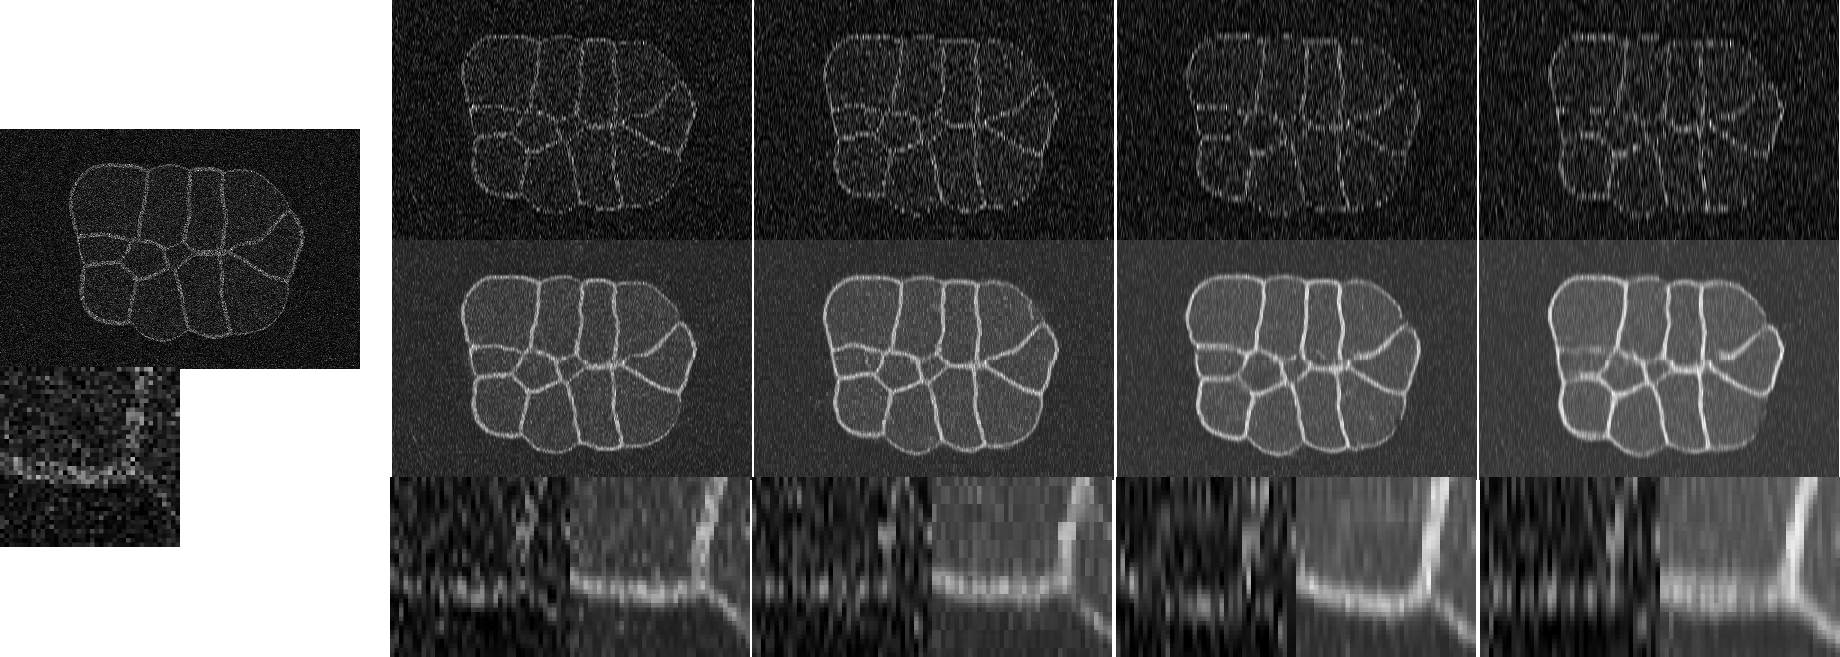
\includegraphics[width=1\columnwidth]{./figures/prediction.png}
    \caption{The five columns show the predicted result of the model with a dilated convolutional layer (filter size 3) and a convolutional layer (filter size 3) for varying k\_factors. From left to right we have: ground truth and enlarged patch (no interpolation) and then four columns in order with k\_factors 3, 4, 5 and 6 where the top image contains the bicubic interpolation of the low resolution axial slice, the middle row contains the prediction for the image above, and the bottom row contains an enlarged (no interpolation) sample patch of the two images above, bicubic interpolation on the right and prediction on the left.}\label{fig:predictions}
\end{figure}

The predicted pictures of model number 3 for k\_factor $\in \{3, 4, 5, 6\}$ can be seen in Figure~\ref{fig:predictions}. We can see clearly that the model manages to enhance the detail of the membranes between the cells compared to the bicubic interpolation. As a side effect, the algorithm also reduces the gaussian noise present in the ground truth, which results in a more contrasted look. In addition to that, all models consistently yield predictions that are noticeably brighter than the ground truth, an effect which seems to worsen for higher k\_factors.

\section{Conclusion}
We have been able to show that the application of the CNN superresolution approach in order to restore axial resolution of anisotropic microscopy imaging data is a promising approach. Our best models have managed to improve the peak noise-to-signal ratio by 1.55dB for a k-factor of 3 and by around 1.9dB for higher k-factors compared to traditional bicubic interpolation. Visual inspection of the results confirms that a significant amount of structure is recovered in the process, suggesting that this method could help further processing of the data such as segmentation.

There are many ways in which this work can be extended and be improved upon. As mentioned in \citet{WEIGERT2017}, taking the point spread function (PSF) into account will be necessary when applying this method to real datasets. Furthermore, as can be seen in Section~\ref{sec:results}, much depends on the choice of hyperparameter values and network architecture. A deeper exploration of the relevant parameter space is likely to reveal significantly better performing and/or more efficient models.

% Mention future work
% - inclusion of PSF
% - further optimization of hyperparameters
% - training and recall of generalized model (multiple training volumes)
% - performance optimizations
% - perform segmentation on augmented images


%----------------------------------------------------------------------------------------
%   BIBLIOGRAPHY
%----------------------------------------------------------------------------------------

\bibliographystyle{plainnat}
\bibliography{report}

%----------------------------------------------------------------------------------------

\end{document}
